\chapter{РОБКО 01}
\section{История}
През 80-те години на 20-ти век в България се наблюдава бурно развитие на електрониката.
\cite{NRB_electronics}
Управляваната от компютри автоматика навлиза все повече в индустрията. Поради нуждата от квалифицирани специалисти по автоматика и мехатроника е създадена серията учебни роботи РОБКО. Представляват неголеми механизми, задвижвани от стъпкови електродвигатели. Наподобяват индустриални роботи. Предназначени са да се управляват от персонален компютър Правец 82 или ИМКО-2.\\
\indent{} %те са еднакви
Серията РОБКО е разработена в Института по Техническа Кибернетика и Роботика към Българската Академия на Науките (ИТКР-БАН) и произвеждана от Завод за медицинса техника в град София. Повечето модели РОБКО са еквиваленти на проектирани в западна Европа и САЩ роботи. Например РОБКО 9 е копие на Heathkit HERO 1, а РОБКО 10 силно наподобява Microbot TeachMover.
\cite{robko-obscomp-history}
Първият робот от серията - РОБКО 01 (показан на фиг. \ref{fig:robko01_mini_mover}) е директно копие на американския робот Mini-mover 5. Той е най-популярният РОБКО, произведени са между 4 и 17 хиляди броя.
\cite{robko-obscomp-history}\\
\indent{}
\begin{figure}
    \centering
    \begin{subfigure}{1\textwidth}
        \centering
        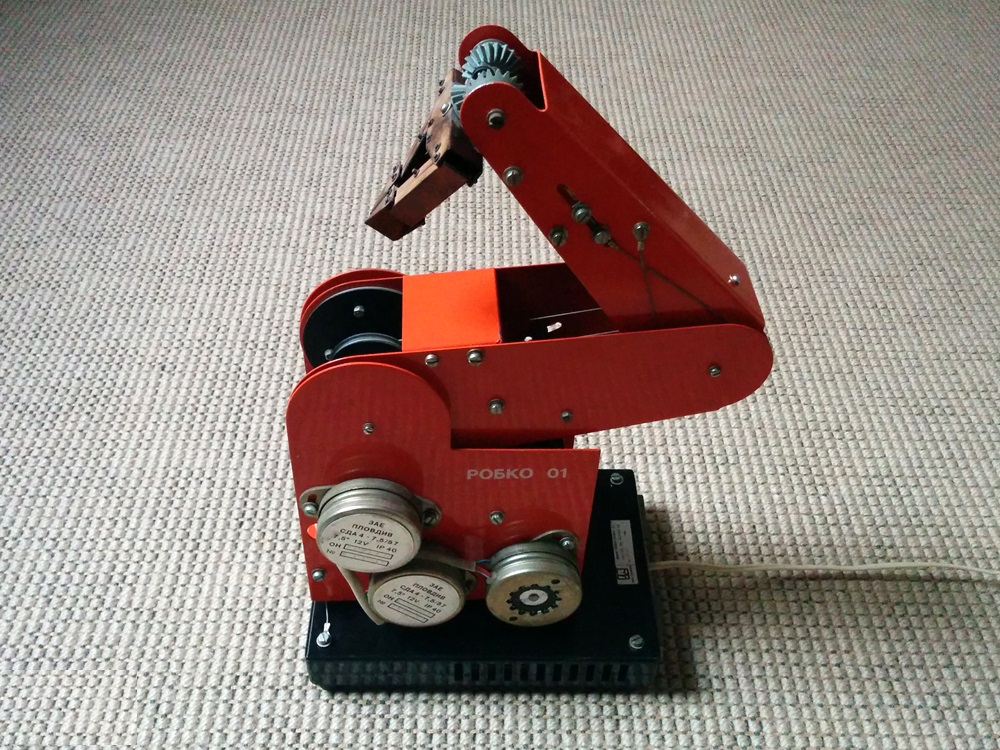
\includegraphics[width=.7\linewidth]{pictures/robko01.jpg}
        \caption{РОБКО 01}
        \label{fig:robko01}
    \end{subfigure}
    \par\bigskip
    \begin{subfigure}{1\textwidth}
        \centering
        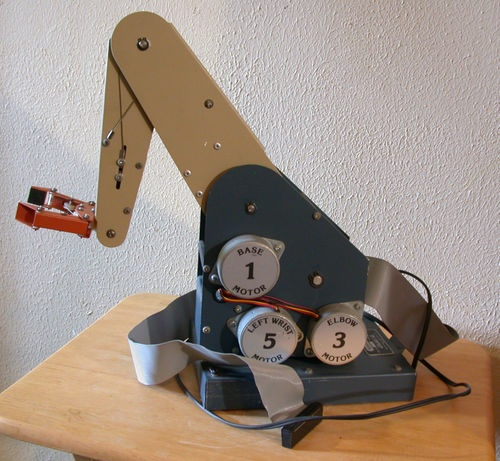
\includegraphics[width=.7\linewidth]{pictures/mini_mover.jpg}
        \caption{Mini-mover 5}
        \label{fig:mini_mover}
    \end{subfigure}
    \caption{РОБКО 01 и Mini-mover 5}
    \label{fig:robko01_mini_mover}
\end{figure}
Серията РОБКО включва въртяща се маса и конвейер (фиг. \ref{fig:turntable}), вариант на РОБКО 01 с монтирани на ставите мотори вместо метални жила за предаване на движението (фиг. \ref{fig:robko_alt}), модел със собствена работна маса (фиг. \ref{fig:robko_vela}), робот с деликатна щипка за стъкленици (фиг. \ref{fig:robko_lab}) и подобен на кран робот (фиг. \ref{fig:collection}, горе-ляво и център-дясно).
\begin{figure}
    \centering
    \begin{subfigure}{0.45\textwidth}
        \centering
        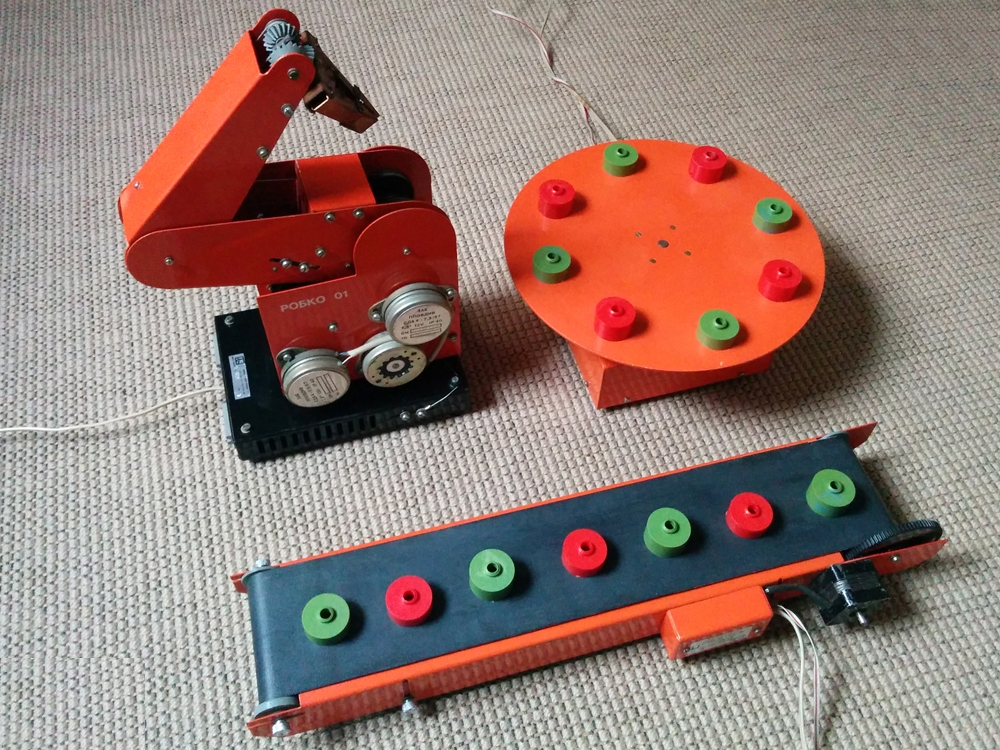
\includegraphics[width=\linewidth]{pictures/turntable_conveyor.jpg}
        \caption{Въртяща се маса и конвейер}
        \label{fig:turntable}
    \end{subfigure}
    \hfill%
    \begin{subfigure}{0.45\textwidth}
        \centering
        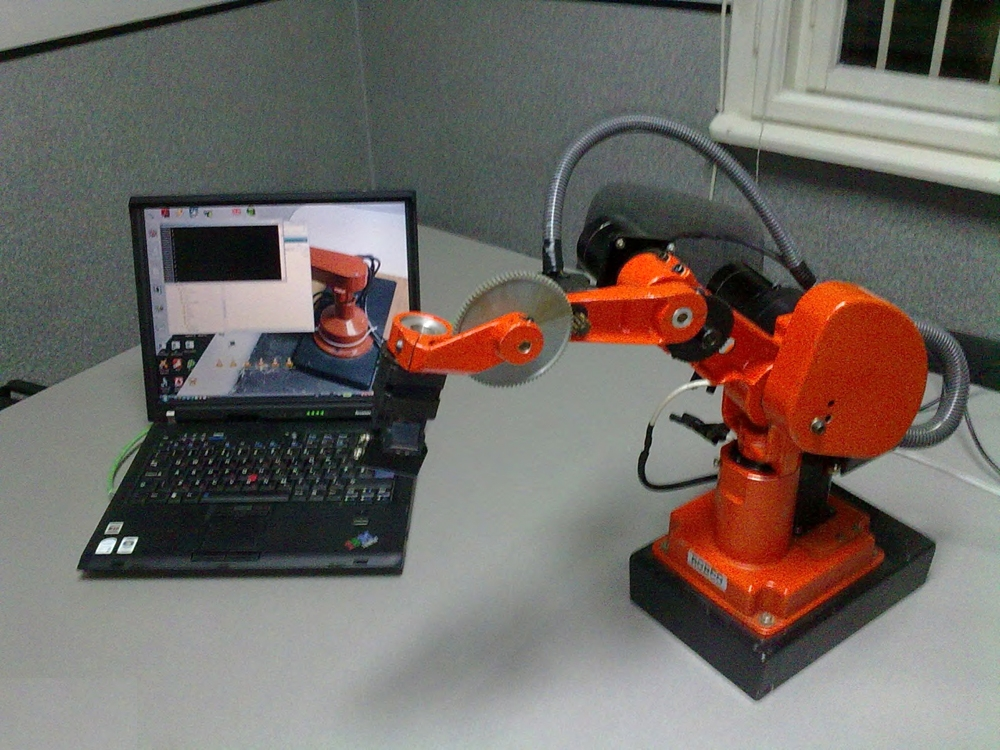
\includegraphics[width=\linewidth]{pictures/robko_alt.jpg}
        \caption{Подобен на РОБКО 01 модел}
        \label{fig:robko_alt}
    \end{subfigure}
    \par\bigskip
    \begin{subfigure}{0.45\textwidth}
        \centering
        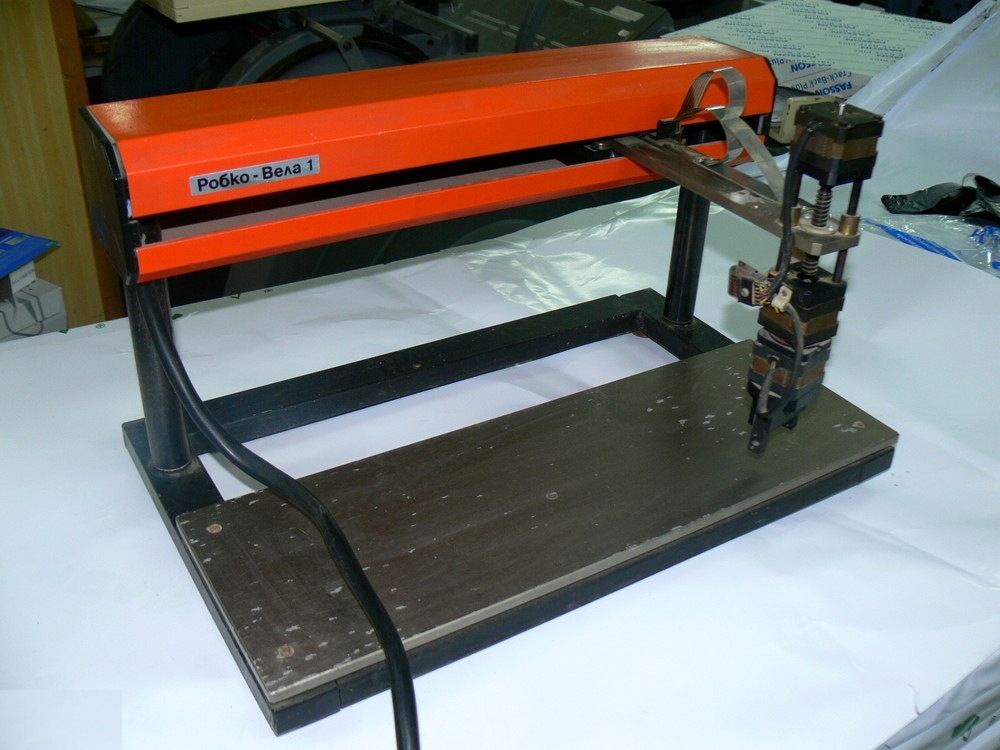
\includegraphics[width=\linewidth]{pictures/robko_vela.jpg}
        \caption{РОБКО Вела 1}
        \label{fig:robko_vela}
    \end{subfigure}
    \hfill%
    \begin{subfigure}{0.45\textwidth}
        \centering
        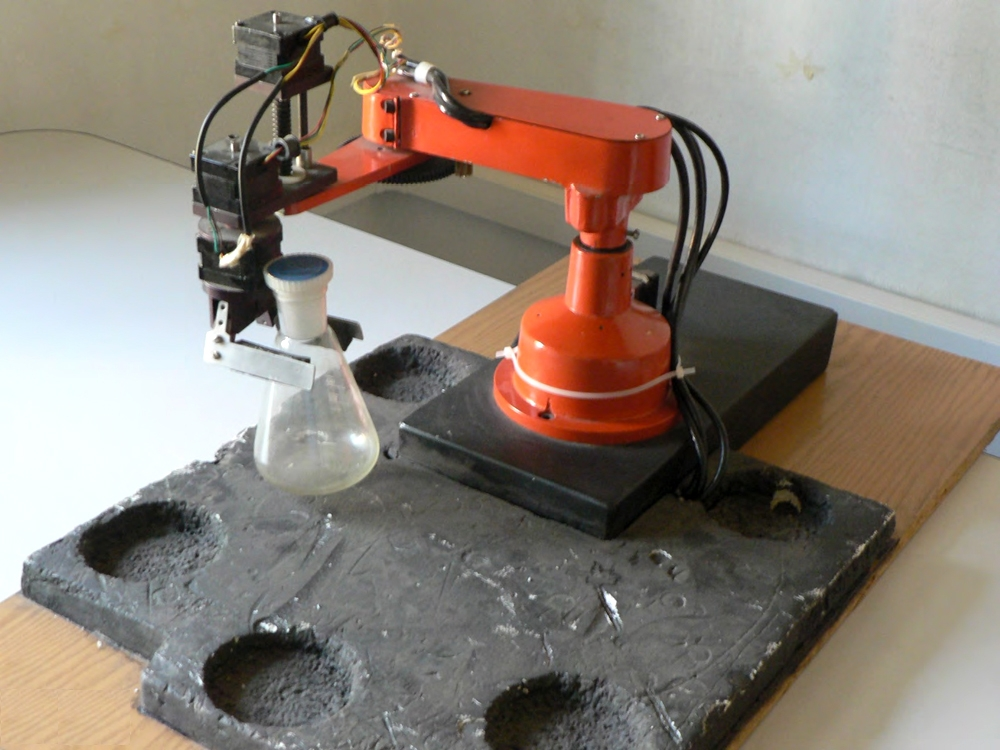
\includegraphics[width=\linewidth]{pictures/robko_lab.jpg}
        \caption{Лабораторен модел}
        \label{fig:robko_lab}
    \end{subfigure}
    \caption{Различни модели от серията РОБКО}
    \label{fig:robko_series}
\end{figure}
\begin{figure}
    \centering
    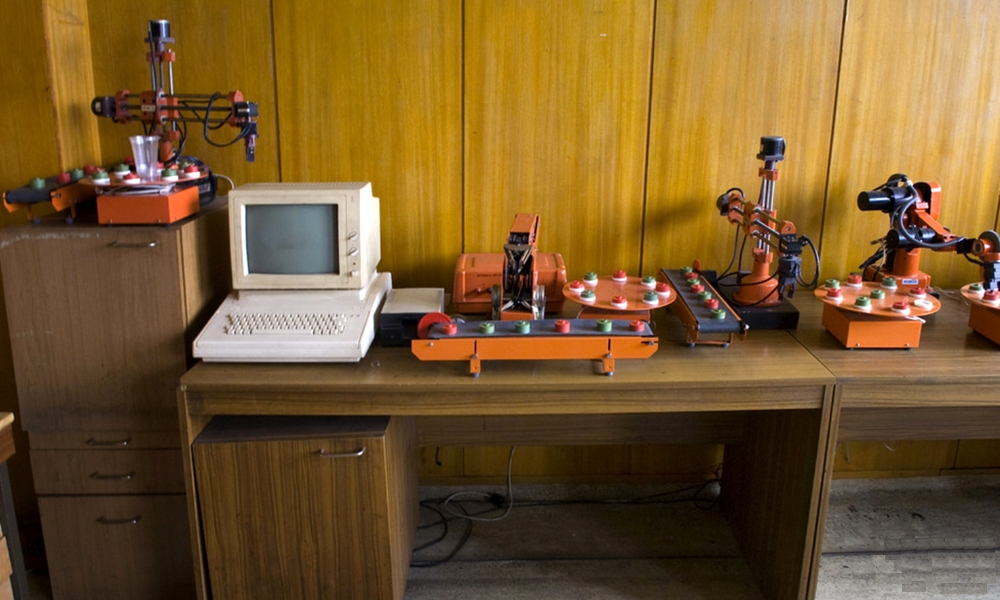
\includegraphics[width=\linewidth]{pictures/robko_collection.jpg}
    \caption{Колекция от различни модели РОБКО и Правец 8М}
    \label{fig:collection}
\end{figure}
Произвеждани са захранващ блок (фиг. \ref{fig:robko_psu}) и три различни накрайника за РОБКО 01 - обикновен хващач, оптичен сензорен хващач (фиг. \ref{fig:robko_opto}) и електромагнит (фиг. \ref{fig:robko_em}). Оптичният сензорен хващач се разглежда подробно в точка \ref{opto_claw_section}.
\begin{figure}
    \centering
    \begin{subfigure}{0.7\textwidth}
        \centering
        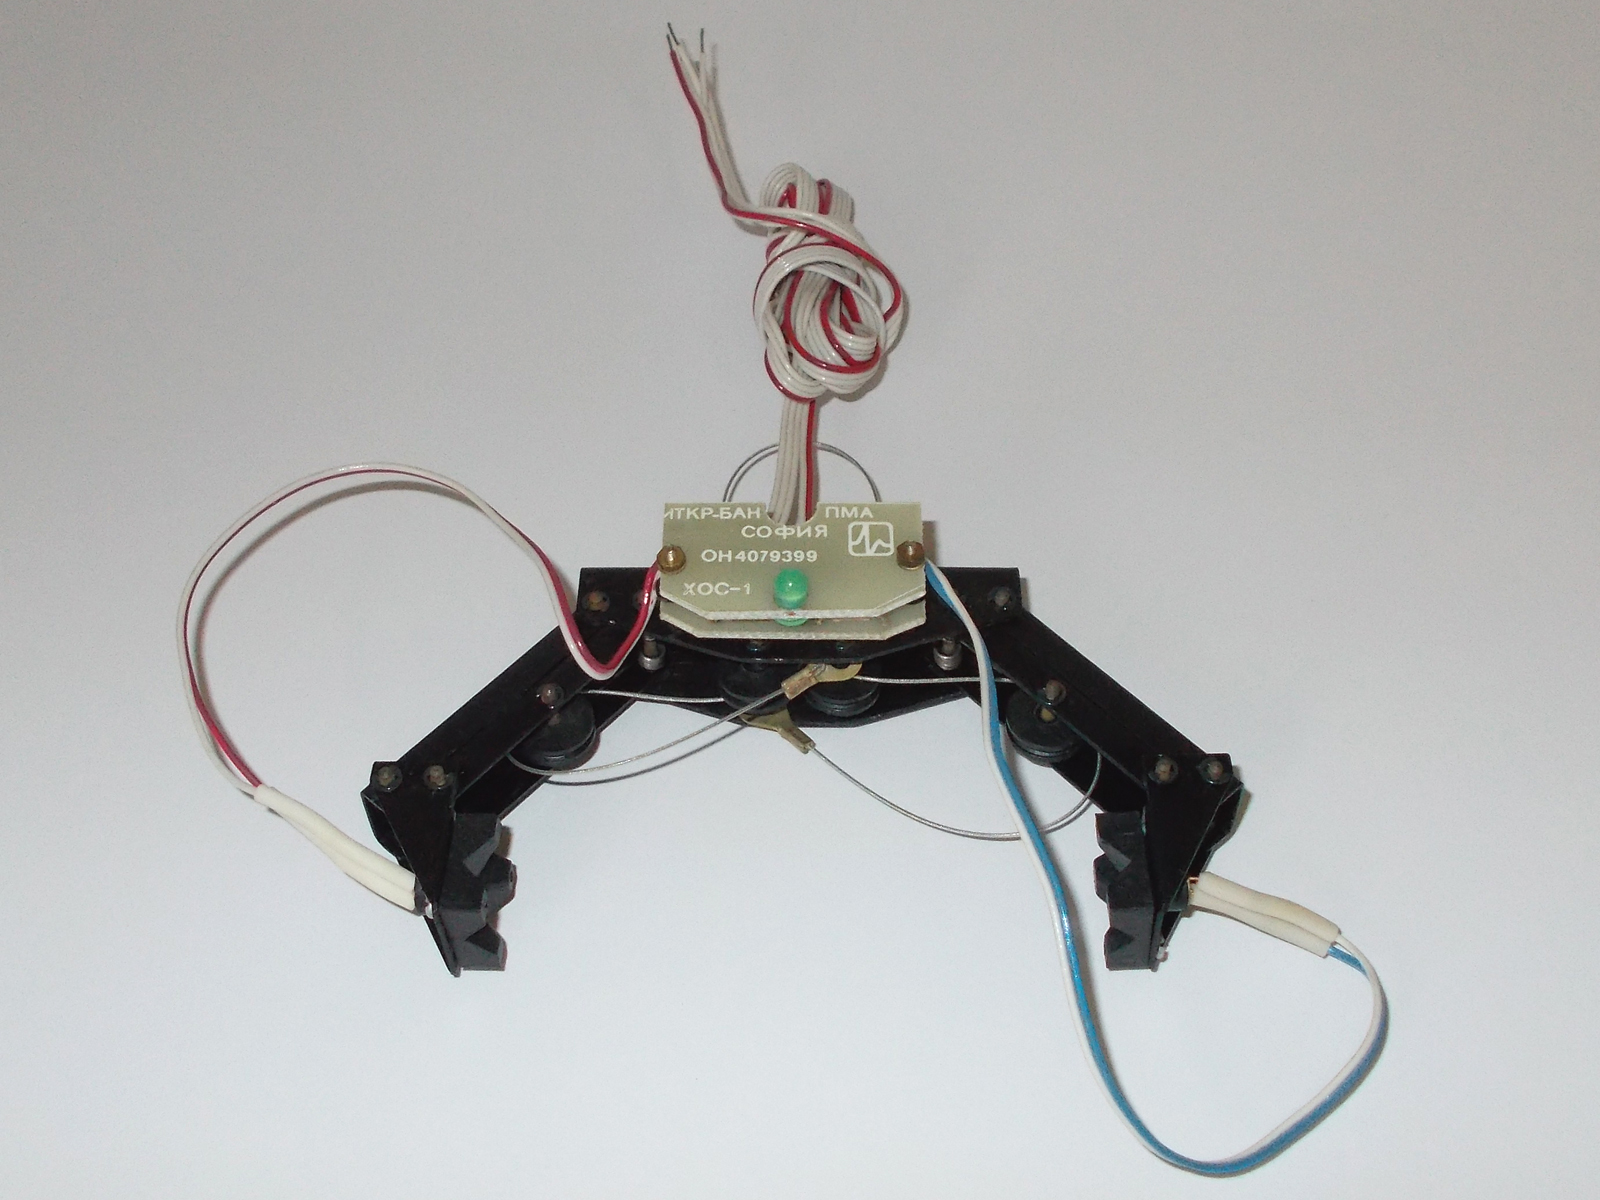
\includegraphics[width=\linewidth]{pictures/robko_opto_claw.jpg}
        \caption{Оптичен сензорен хващач}
        \label{fig:robko_opto}
    \end{subfigure}
    \par\bigskip
    \begin{subfigure}{0.45\textwidth}
        \centering
        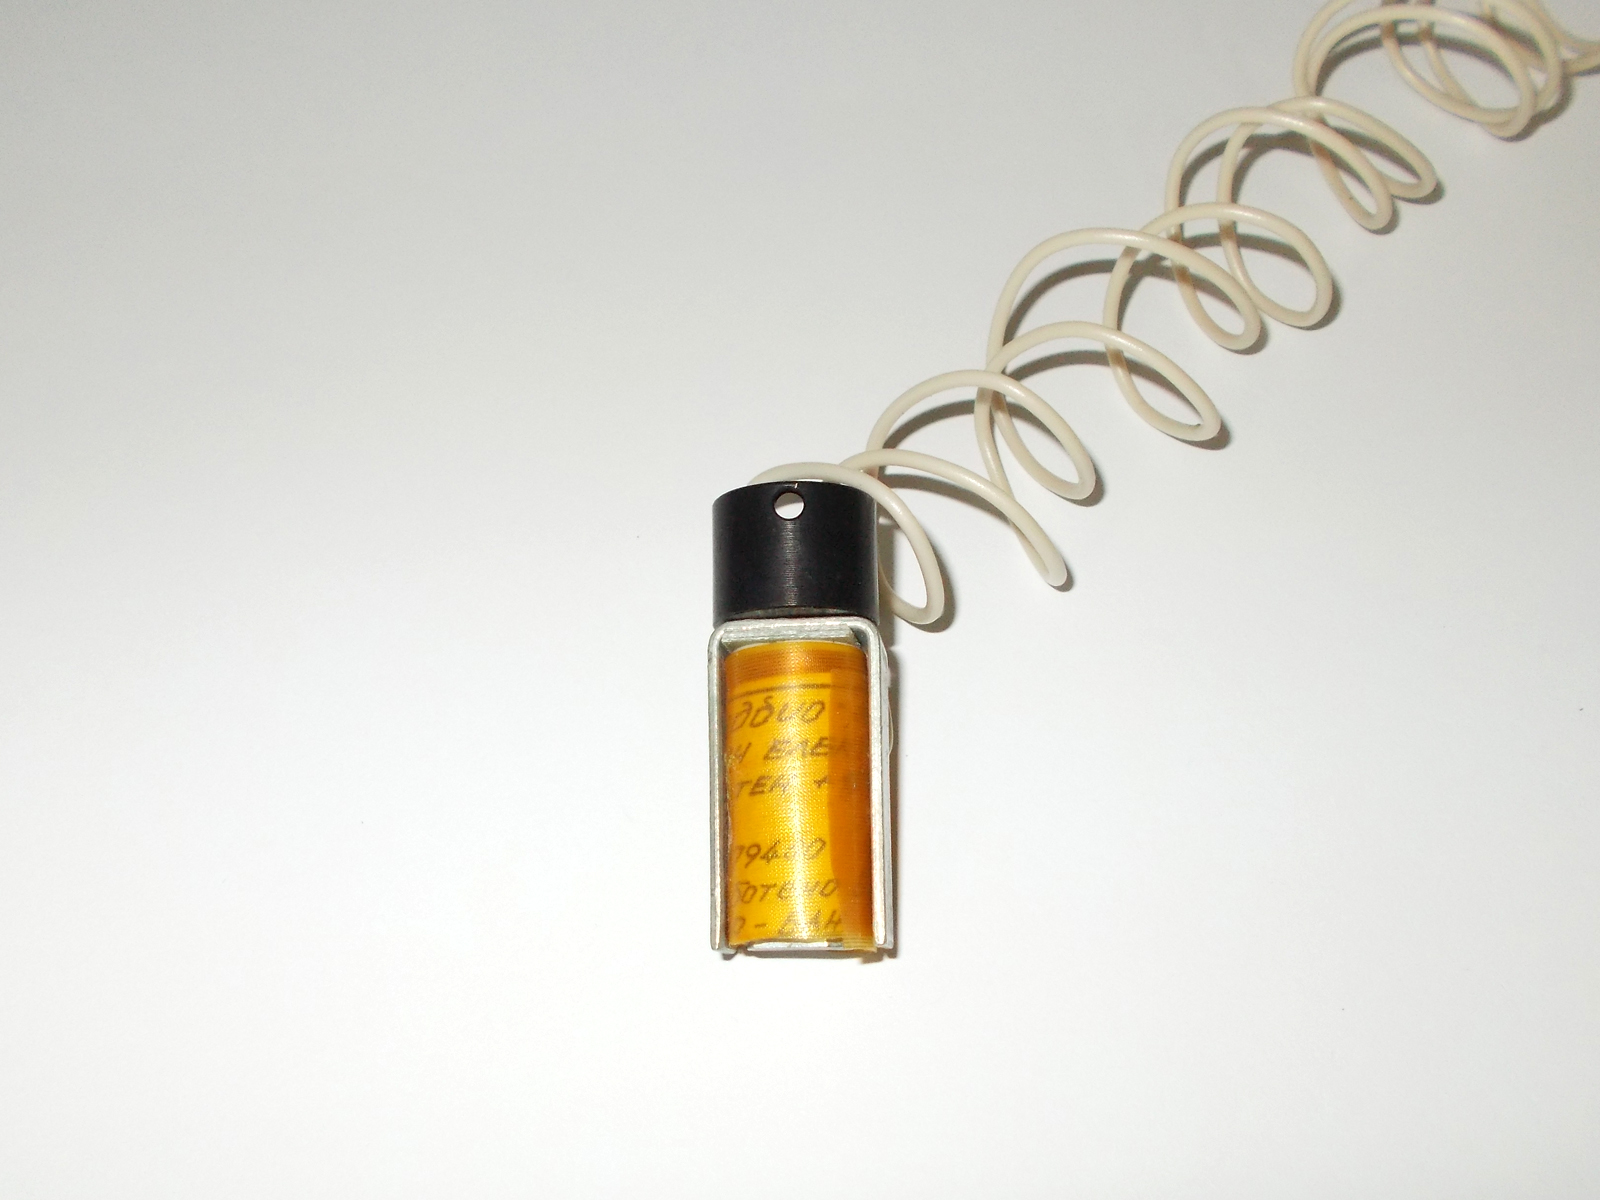
\includegraphics[width=\linewidth]{pictures/robko_electromagnet.jpg}
        \caption{Електромагнит}
        \label{fig:robko_em}
    \end{subfigure}
    \hfill%
    \begin{subfigure}{0.45\textwidth}
        \centering
        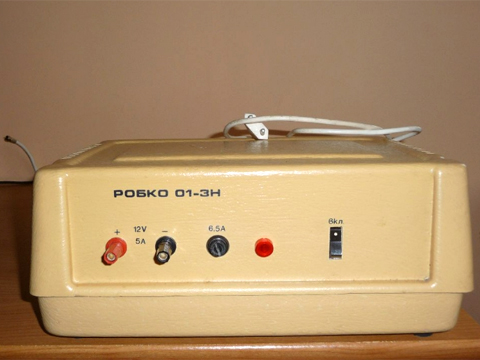
\includegraphics[width=\linewidth]{pictures/robko_psu.jpg}
        \caption{Захранващ модул}
        \label{fig:robko_psu}
    \end{subfigure}
    \caption{Аксесоари за РОБКО 01}
    \label{fig:robko_accessories}
\end{figure}
\section{РОБКО 01 в настоящето}
Малкото запазени екземпляри от серията РОБКО почти винаги са от модел 01 или комплект въртяща се маса и конвейер. Съществуват различни проекти, успешно реализирали управление на РОБКО 01. Някои от тях се свързват с драйверната платка на робота, а други я заменят. Разработени са различни потребителски интерфейси: програми с графична среда, програми с команден ред и управление с джойс
тици.\\\indent{}
РОБКО 01 е проектиран да се управлява от ИМКО-2/Правец82 чрез разширителната карта показана на фигура \ref{fig:orig_cntrl}. Повечето модерни РОБКО проекти заменят тази платка с микроконтролер.\\
\begin{figure}
    \centering
    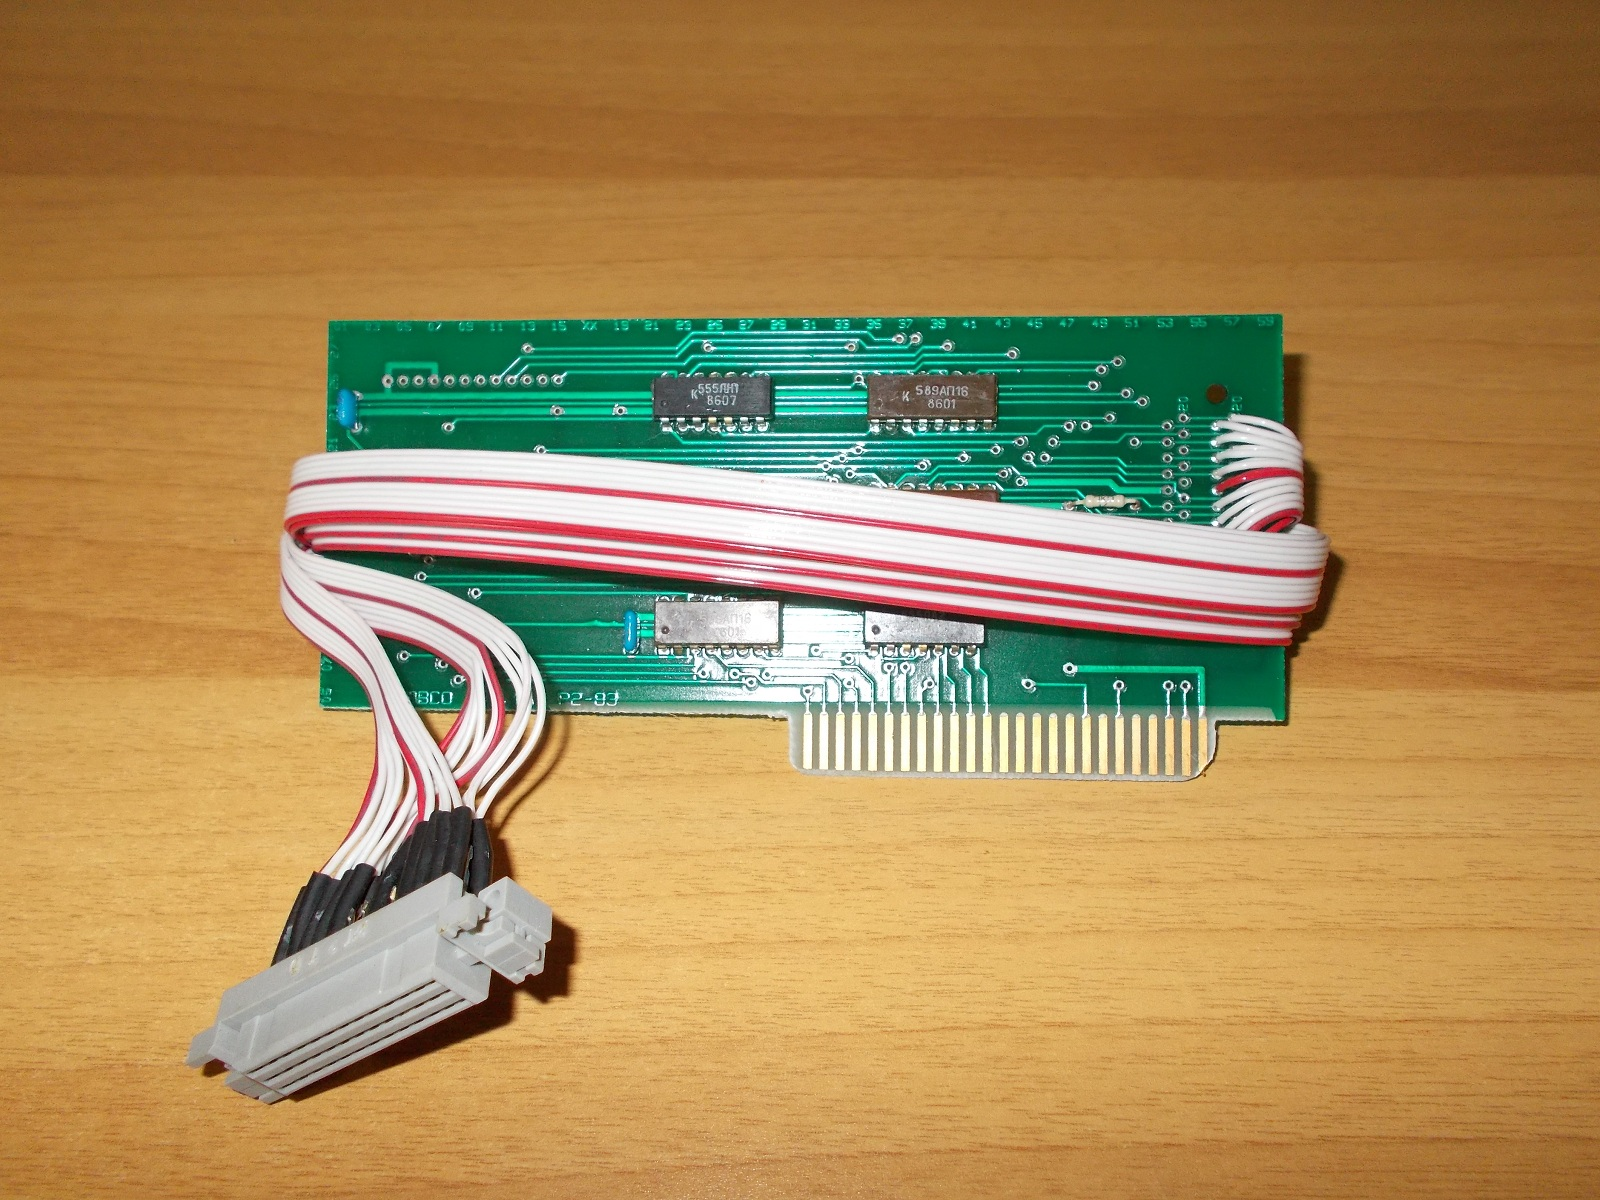
\includegraphics[width=\linewidth]{pictures/robko_orig_controller.jpg}
    \caption{Разширителна карта за ИМКО-2/Правец82, свързваща се с драйверната платка на РОБКО 01}
    \label{fig:orig_cntrl}
\end{figure}

Пример за такава реализация е проектът на Валентин Николов.
\cite{robko-val_niko}
Проектираната от него платка (фиг. \ref{fig:usb_cntrl}) е базирана на микроконтролер PIC4620 от Microchip. Разполага с бутони за ръчно управление и връзка с компютър през USB интерфейс. Неговият софтуер, изпълняван на персонален компютър, предоставя графична среда за управление на робота. Може да се контролира от мишка, клавиатура или джойстик и позволява едновременно движение на повече от един мотор. Демонстрация на функционалностите на проекта на Валентин Николов е налична в интернет.\cite{robko-usb-gui}
\begin{figure}
    \centering
    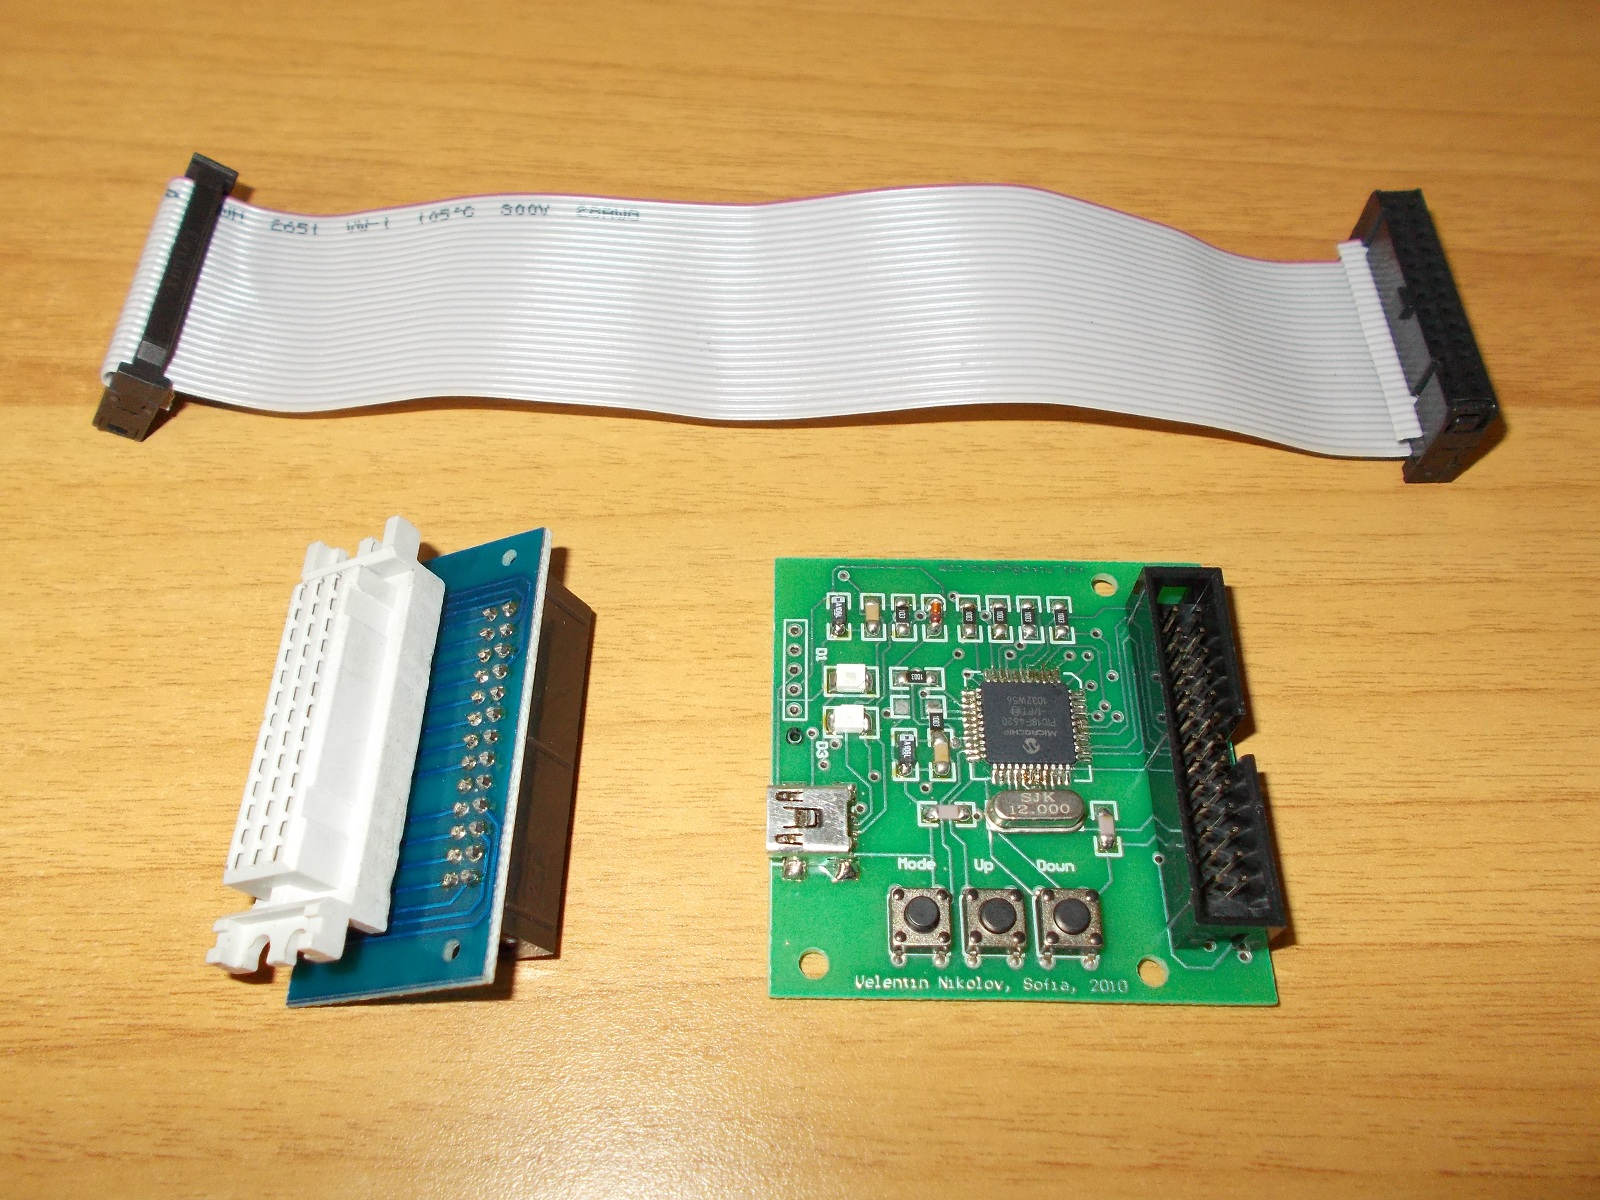
\includegraphics[width=\linewidth]{pictures/robko_usb_controller.jpg}
    \caption{Микроконтролерна платка, свързваща драйверната платка на РОБКО 01 с персонален компютър}
    \label{fig:usb_cntrl}
\end{figure}

Подобна система е разработена от Орлин Димитров - студент в Технически Университет - Габрово. Контролерът, използван от него, е Arduino UNO. Микроконтролерната платка се свързва към РОБКО 01 и към персонален компютър, подаващ команди през серийна връзка. Роботът се управлява от програма с графична среда, изпълнявана на персоналния компютър. Софтуерът позволява както ръчно управление, така и изпълнение на поредица от предварително зададени движения. Отличителна черта на тази система е способнастта й плавно да ускорява и забавя въртенето на моторите.
\cite{robko-orlin-fb}
Проектът на Орлин Димитров е единственият известен в интернет, успешно реализирал едновременното управление на повече от един РОБКО 01.
\cite{robko-orlin-double2}

Друг подход за управлението на РОБКО 01 е да се подмени драйверната платка на робота. Този метод е приложен от Симеон Иванов, студент от Русенският университет "Ангел Кънчев".
\cite{robko-atmega128}
Разработената от него платка (показана на фигура \ref{fig:new_cntrl_brd}) се монтира на мястото на оригиналната драйверна платка в основата на робота. Включва в себе си микроконтролер ATMega128, Ethernet контролер ENC424J600, захранващ блок, шест интегрални схеми за управление на стъпкови мотори и интегрални схеми за комуникация по UART, RS232 и USB. Тази разработка е най-функционалната имплементация на РОБКО 01 сред известните в интернет такива.\\
\indent{}
Контролерът комуникира с персонален компютър по ModBUS протокол, който е стандартен за автоматизацията в индустриални условия. Това позволява отдалечено управление на робота по интернет. Могат да се движат множество мотори едновременно. Софтуерът на микроконтролерът извършва изчисления за права и обратна кинематика - може да позиционира щипката на робота на зададени координати и да определя текущото местоположение. Командите към контролера се подават под формата на G код. Това на практика превръща РОБКО 01 в CNC (Цифрово-Програмно Управляема) машина. Тази способност на разработката е показана на видеоклип в интернет.
\cite{robko-cnc}
\begin{figure}
    \centering
    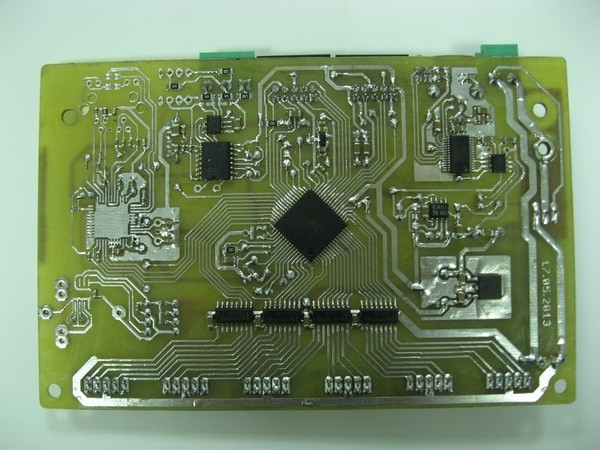
\includegraphics[width=\linewidth]{pictures/robko_new_driver_board.jpg}
    \caption{Платка, заменяща оригиналната драйверна платка на РОБКО 01}
    \label{fig:new_cntrl_brd}
\end{figure}
\section{Настояща разработка}
Целта на настоящия проект е да се проектира и изработи управляващо устройство за РОБКО 01 базирано на микроконтролер STM32L476RG Nucleo. Основните възможности на РОБКО 01 вече са реализирани в гореспоменатите разработки. Устройството, разглеждано в тази дипломна работа, се отличава със способността да засича предмети чрез оптичния сензорен хващач. Няма известна в интернет разработка, успешно реализираща тази функционалност на РОБКО 01. Това се дължи до голяма степен на малкият брой оцелели до днес оптични сензорни хващачи за РОБКО 01.\\
\indent{}
Ключово внимание в текущата работа е обърнато на управлението по интернет. Други важни функционалности са изпълнението на команди, предварително записани във файл и буферирането на получените команди. Реализиран е и ръчен контрол чрез джойстици.\\
\indent{}
Не е разработена графична среда, понеже функционалностите които би предоставила биха се застъпвали с ръчното управление и софтуерът за отдалечено управление. Предвидени са възможности за движение по координати и запомняне на позиции, но не са реализирани на днешна дата.
\section{Тенденции в автоматизацията}
Вследствие на бурното развитие на компютърните мрежи все повече устройства разполагат с мрежова свързаност. Практиката да се добавя способност за комуникация през интернет в разнообразни уреди е известна като "Интернет на вещите". Това позволява множество уреди, поначало неразполагащи с мрежова свързаност, да комуникират по между си, с хора и с централен възел или сървър. Реализира се с помощта на вградени микроконтролерни системи и мрежови технологии, нерядко безжични.
\cite{IoT-def}\\
\indent{}
На базата на тази концепция се изграждат системи за автоматизация и управление, често в домашни условия. Такива системи се състоят от съвкупност от сензори (температура, светлина, натиск и много други), изпълнителни устройства (мотори, климатици, лампи и др.) и управляващи устройства (компютър, микроконтролер).
\cite{home-auto-def}
В близкото бъдеще е възможно сложни системи за домашна автоматизация да се интегрират с цифрови асистенти като Google Home и Amazon Echo.\\
\indent{}
Комютрите отдавна се използват в идустрията за автоматизация, но с ограничена комуникация между отделните машини. Навлизането на модерните мрежови технологии в индустрията позволява по-бърз обмен на големи количества данни и по-голяма взаимосвързаност между машините. Това е една от предпоставките за настъпващата четвърта индустриална революция.
\cite{industry-4.0}\\
\indent{}
Заводите на новото време ще се нуждаят от все по-малка човешка намеса. Когато има нужда от такава, в много случаи може да се извършва отдалечено чрез подходящи мрежови технологии. С оглед на това текущата разработка не цели единствено да реставрира музеен експонат от времето на социалистическа България, а да демонстрира нагледно възможността за отдалечено управление на индустриални машини.\\
\indent{}
Пример за отдалечено управление на завод е показан на фигура \ref{fig:example_use}. Заводът разполага с множество машини, всяка с вграден микроконтролер. Индустриален компютър е свързан към контролерите на машините съставящи една поточна линия или сегмент от такава. Компютърът съгласува действията на отделните машини и разполага с връзка към Интернет. Ресурсите на завода могат да се разширят като се добавят нови групи от машини и компютри. Операторът на машините може да работи в офис далеч от сградата на завода и да управлява производствения процес от там.
\begin{figure}[!htb]
    \centering
    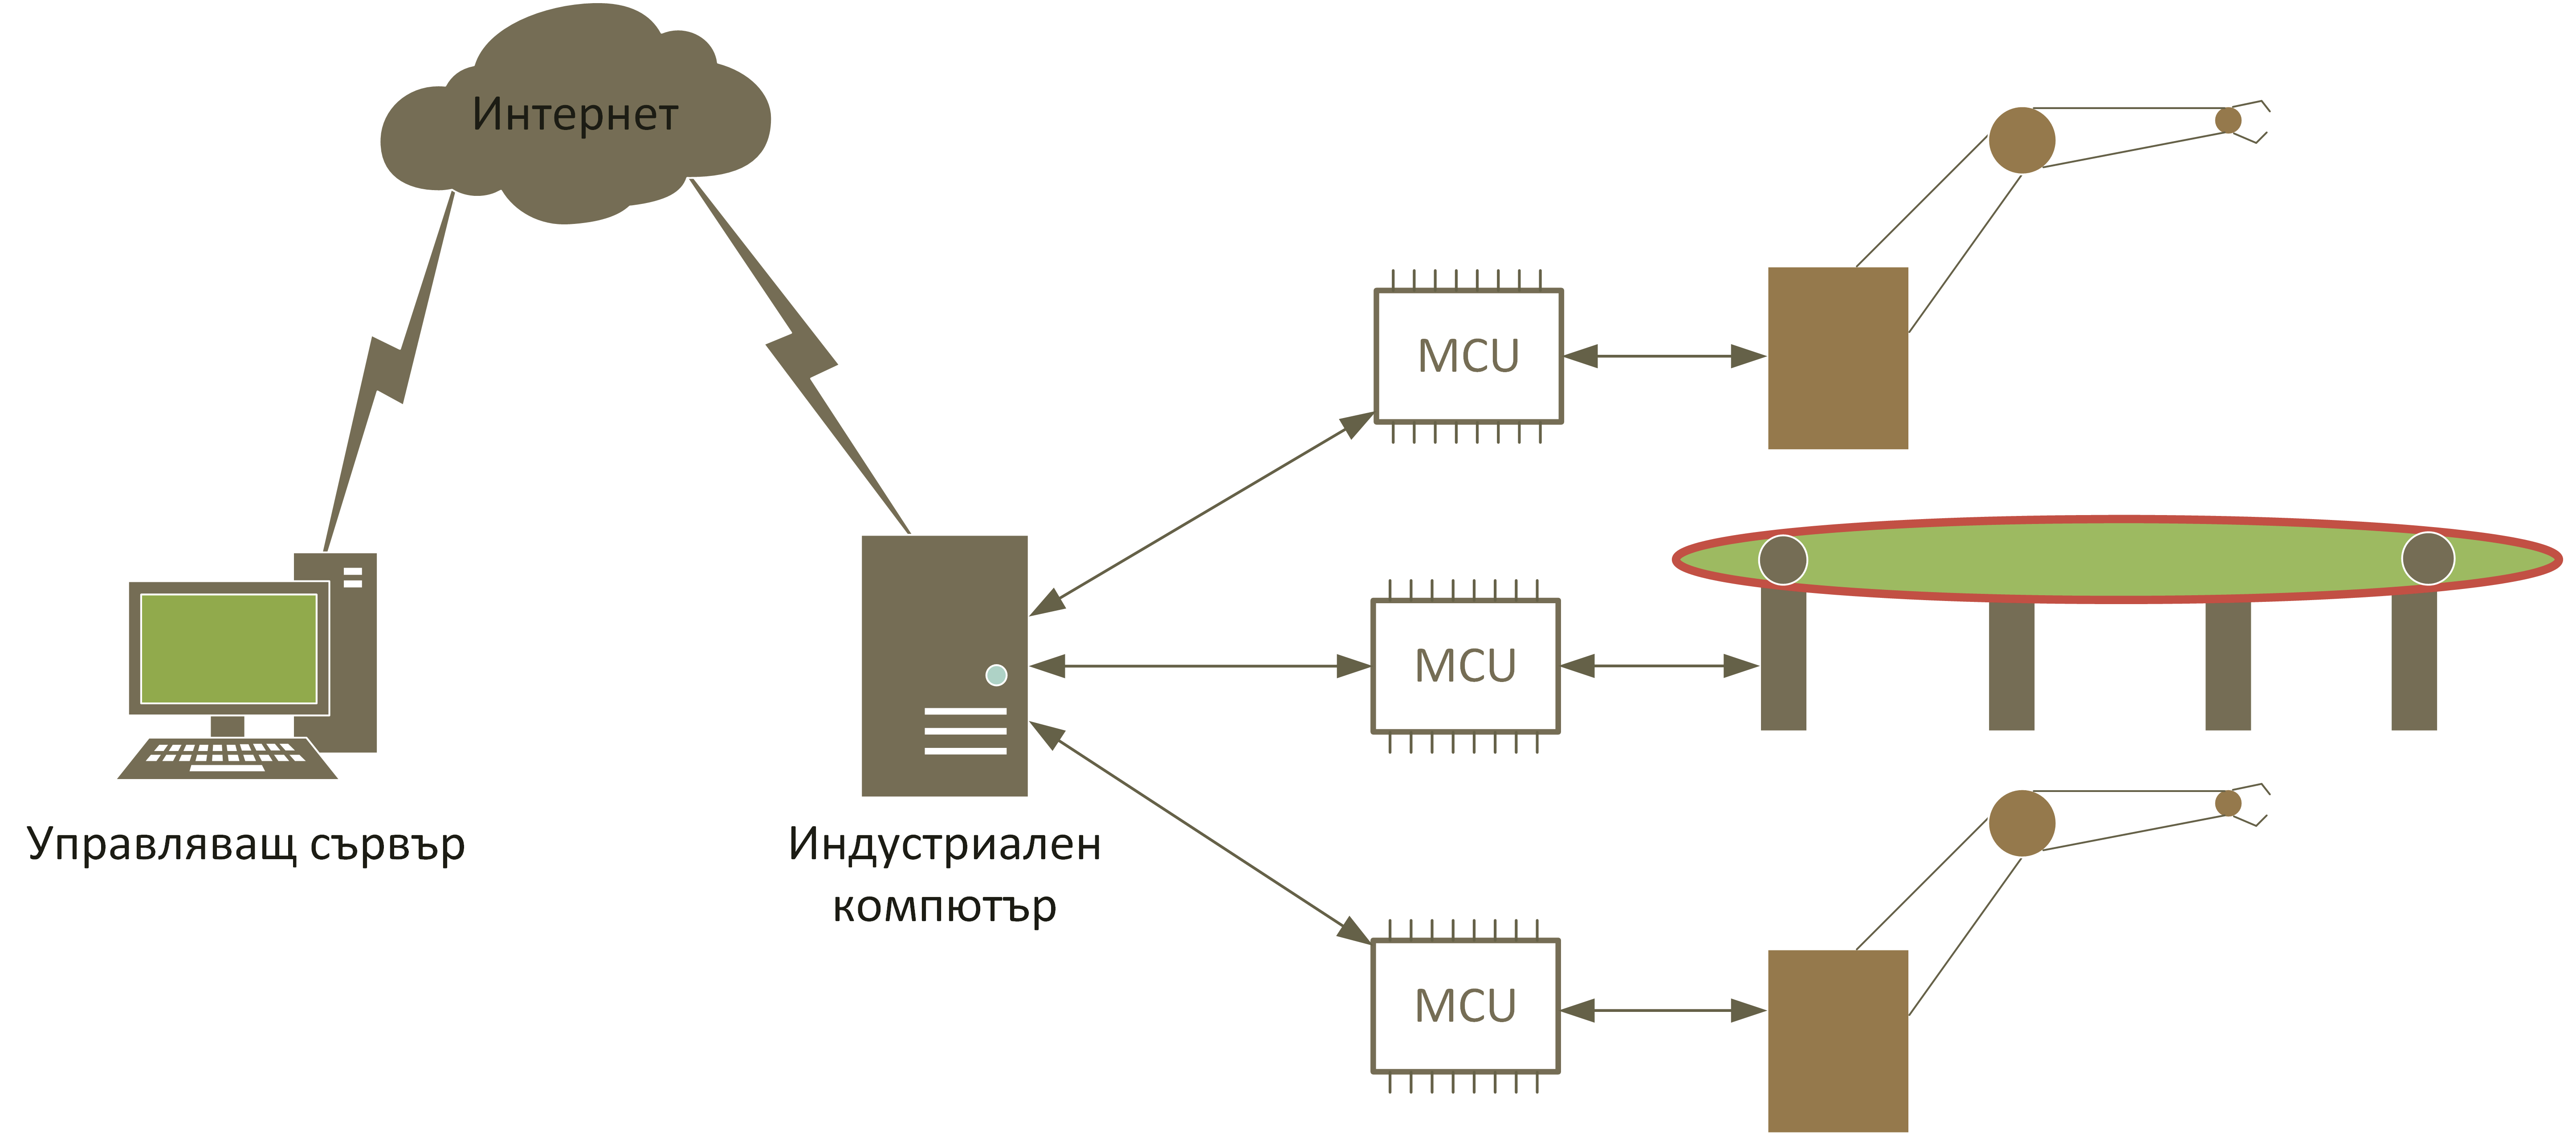
\includegraphics[width=\linewidth]{pictures/ROBKO_example_use.png}
    \caption{Пример за отдалечено управление на поточна линия}
    \label{fig:example_use}
\end{figure}